\documentclass{aastex}
%\documentclass{article}
\usepackage{graphicx}
%\usepackage{natbib}   
\bibliographystyle{apj}
%\bibliographystyle{plain}

\begin{document}

\title{Paper Summary}
\author{Laurel Farris}

\maketitle

A discussion of observations of emission from NGC 253, a starburst galaxy
about 3.44 Mpc away, is presented \cite{paper}. Evidence of star formation 
can be detected with both thermal emission and the H40$\alpha$ emission line.
At the millimeter wavelengths oberved here, both star formation and possibly 
electron temperatures can be constrained. Figure 
%\ref{wrongimage} 
shows some of the 
observations obtained of this galaxy at the center.

%\begin{figure}[here]
%    \centering
%    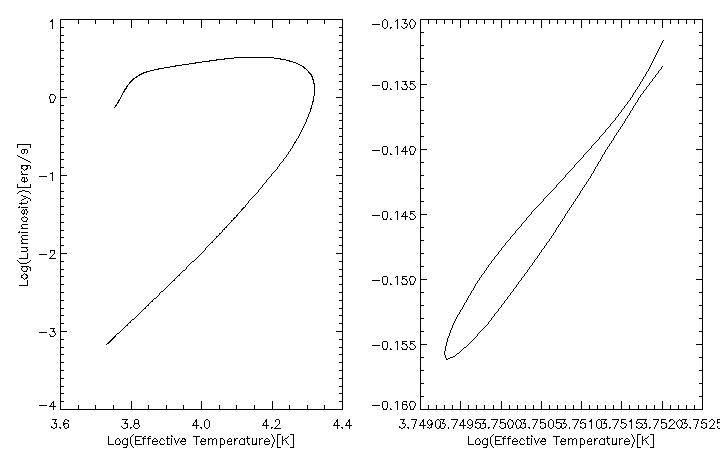
\includegraphics[width=5.0in]{fig2.jpg}
%    \caption{These three images are of the center of NGC 253. The first
%               shows the continuum brightess, the middle is the H40$\alpha$
%               line intensity, and the third is the H40$\alpha$ velocity.}
%    \label{wrongimage}
%\end{figure}


The three key results from this paper were:
\begin{enumerate}
    \item The electron temperature was measured.
    \item Numbers for the star formation rate and Q were obtained.
    \item The galaxy was found to have more dust than previously thought,
            so NIR observations should be used with caution.
\end{enumerate}

\bibliography{reffile}

\end{document}
